\section{Homework 9}

\subsection{Bus Arrivals At Cory Hall}
(a) This is just $Poisson(\mu x)$. That is, 
\[
\P[\text{\# of students} = k] = \frac{(\mu x)^k e^{-\mu x}}{k!}
\]

(b) Suppose we are given that $k$ students have already arrived and are waiting for the next bus. Due to the memoryless property, the distribution of the arrival time for the bus is still exponentially distributed with parameter $\lambda$ and the arrival time for the next student is exponentially distributed with parameter $\mu$. We have shown in the past that the probability of one exponential hitting before another is just $\frac{\mu}{\lambda + \mu}$. It follows then that the distribution of the number of students to get on the next bus is geometrically distributed with parameter $\frac{\lambda}{\lambda + \mu}$. That is, $Geom\left(\frac{\lambda}{\lambda + \mu}\right)$.

(c) Let $N = N_{\f{before}} + N_{\f{after}}$, splitting arrivals between those before and after 9:30. Note $N_{\f{before}} \sim N_{\f{after}} \sim Geom(\frac{\lambda}{\lambda + \mu})$. Then we find the distribution of $N$ to be
\begin{align*}
    \P[N = k] &= \sum_{i = 0}^k\P[N_{\f{before}} = i]\P[N_{\f{after}} = k - i] \\
        &= \sum_{i = 0}^k\left(\frac{\lambda}{\lambda + \mu}\right)\left(\frac{\mu}{\lambda + \mu}\right)^i\left(\frac{\lambda}{\lambda + \mu}\right)\left(\frac{\mu}{\lambda + \mu}\right)^{k - i} \\
        &= (k + 1)\left(\frac{\lambda}{\lambda + \mu}\right)^2\left(\frac{\mu}{\lambda + \mu}\right)^k.
\end{align*}


\subsection{Basketball II}
Let $a_i$ be the probability of winning from state $i$, where the states are from the set $\{-k, -(k - 1), \dots, -1, 0, 1, \dots, k-1, k\}$. Let $p = \frac{\lambda_A}{\lambda_A + \lambda_B}$. Then we have the following system of equations
\begin{align*}
    a_{-k} &= 0 \\
    a_{i} &= pa_{i + 1} + (1 - p)a_{i - 1} \qquad \text{ for $-k < i < k$} \\
    a_k &= 1.
\end{align*}
We rewrite the second one as
\[
(1 - p)(a_i - a_{i - 1}) = p(a_{i + 1} - a_i).
\]
Letting $\delta_i = a_{i + 1} - a_i$ and $\rho = \frac{1 - p}{p}$, we have
\[
\delta_i = \rho^i\delta_0 = \rho^{i + k}\delta_{-k}
\]
Note that $\delta_{-k} + \delta_{-(k - 1)} + \dots + \delta_{k - 1} = a_k - a_{-k} = 1$, we see that 
\[
\delta_{-k} = \frac{1}{1 + \rho + \dots + \rho^{2k - 1}}
\]
We want to find 
\begin{align*}
    a_0 &= \delta_{-k} + \dots + \delta_{-1} \\
        &= \delta_{-k}(1 + \rho + \dots + \rho^{k - 1}) \\
        &= \frac{1 + \rho + \dots + \rho^{k - 1}}{1 + \rho + \dots + \rho^{2k - 1}}
\end{align*}
which becomes
\[
a_0 = 
\begin{cases}
    \frac{1 - \rho^k}{1 - \rho^{2k}}, &\text{ if $\rho \neq 1$} \\
    1/2, &\text{ if $\rho = 1$}
\end{cases}
\]
Substituting $\lambda_A$ and $\lambda_B$ back in, we get
\[
a_0 = 
\begin{cases}
    \frac{1 - (\lambda_A/\lambda_B)^k}{1 - (\lambda_A/\lambda_B)^{2k}}, &\text{ if $\lambda_A \neq \lambda_B$} \\
    1/2, &\text{ if $\lambda_A = \lambda_B$}
\end{cases}
\]


\subsection{Frogs}
(a) Let $\pi_i$ denote the stationary probability of $i$ frogs being on land. We have the balance equations:
\begin{align*}
    6\pi_0 &= \pi_1 \\
    5\pi_1 &= 6\pi_0 + 2\pi_2 \\
    4\pi_2 &= 4\pi_1 + 3\pi_3 \\
    3\pi_3 &= 2\pi_2.
\end{align*}
Solving and normalizing, we get
\[
    \pi = \left[\frac{1}{27}, \frac{6}{27}, \frac{12}{27}, \frac{8}{27}\right]
\]

% Let $X$ be the long run number of frogs in the sun. Then $3 - X$ is the long run number of frogs in the lake. We have
% \[
% X = 2(3 - X),
% \]
% which gives us $X = 2$. That is, on average in the long run there will be 2 frogs in the sun and 1 frog in the lake.

(b) Each frog is an independent 2 state CTMC with the balance equations:
\begin{align*}
    \pi'_S &= 2\pi'_W \\
    \pi'_S + \pi'_W &= 1,
\end{align*}
solving we obtain $\pi' = \left[\frac{2}{3}, \frac{1}{3}\right]$. Then we find $\pi$ from the previous part:
\begin{align*}
    \pi_0 &= \left(\frac{1}{3}\right)^3 = \frac{1}{27} \\
    \pi_1 &= 3\left(\frac{1}{3}\right)^2\left(\frac{2}{3}\right) = \frac{6}{27} \\
    \pi_2 &= 3\left(\frac{1}{3}\right)\left(\frac{2}{3}\right)^2 = \frac{12}{27} \\
    \pi_3 &= \left(\frac{2}{3}\right)^3 = \frac{8}{27},
\end{align*}
which indeed matches what we got in part (a).

\subsection{Taxi Queue}
We model this as a CTMC with four states $\{0, 1, 2, 3, 4\}$ each denoting the number of people waiting at the street corner. We find the stationary distribution using balance equations:
\begin{align*}
    \pi_0 &= 2\pi_1 \\
    3\pi_1 &= \pi_0 + 2\pi_2 \\
    3\pi_2 &= \pi_1 + 2\pi_3 \\
    3\pi_3 &= \pi_2 + 2\pi_4 \\
    2\pi_4 &= \pi_3 \\
    \pi_0 + \pi_1 + \pi_2 + \pi_3 &= 1.
\end{align*}
Solving, we obtain $\pi = \left[\frac{16}{31}, \frac{8}{31}, \frac{4}{31}, \frac{2}{31}, \frac{1}{31}\right]$. Since we are given that he joins the queue successfully, we remove the last probability and normalize to get $\left[\frac{8}{15}, \frac{4}{15}, \frac{2}{15}, \frac{1}{15}\right]$. Now, we find the total expected waiting time, conditioned on the stationary distribution probabilities:
\begin{align*}
    \frac{8}{15} \cdot \frac{1}{2} + \frac{4}{15} \cdot \frac{2}{2} + \frac{2}{15} \cdot \frac{3}{2} + \frac{1}{15} \cdot \frac{4}{2} &= \frac{13}{15}.
\end{align*}
So his expected waiting time will be $13/15$ minutes.

\subsection{Two Server System}

Let $\pi_i$ denote the long term probability of there being $i$ working machines. We have the following balance equations:
\begin{align*}
    \mu \pi_2 &= \lambda \pi_1 \\
    (\mu + \lambda)\pi_1 &= \mu\pi_2 + \lambda\pi_0 \\
    \lambda\pi_0 &= \mu\pi_1.
\end{align*}
Solving and normalizing, we get that $\pi_0 = \frac{\mu^2}{\lambda^2 + \lambda\mu + \mu^2}$.


\subsection{Poisson Queues}
(a) Each state is the number of people currently in the queue. The chain advances to the right at rate $\lambda$ since another person arrives with exponential parameter $\lambda$. The chain advances to the left at rate $n\mu$, where $n$ is the state it is at, since the first person to be finished serving is the the merging of $n$ Poisson processes.
\[
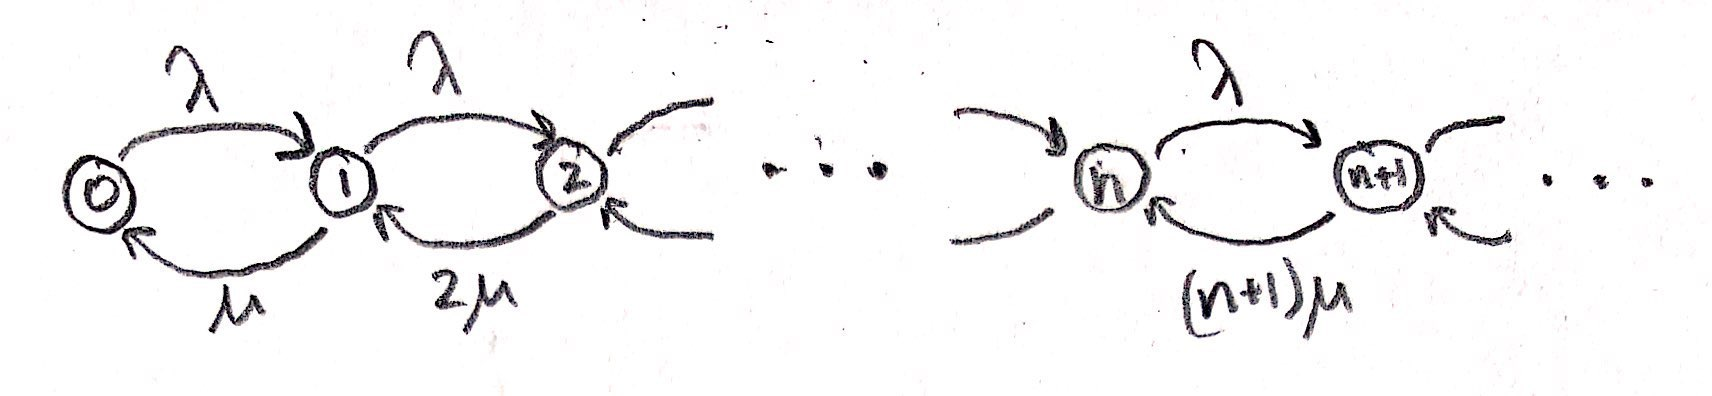
\includegraphics[scale=0.15]{poisson_chain.jpg}
\]

(b) Since an irreducible infinite markov chain is positive recurrent if and only if it has a stationary distribution, it is sufficient to find the stationary distribution. We have the generalized balance equation:
\[
(\lambda + n\mu)\pi_n = \lambda\pi_{n - 1} + (n + 1)\mu\pi_{k + 1}
\]
We claim that $\pi_n = \frac{(\lambda / \mu)^n}{n!}\pi_0$ satisfies these balance equations. Indeed, plugging it in we get equality. Then, normalizing, we get that
\begin{align*}
    \pi_0 &= \frac{1}{e^{\lambda / \mu}} \\
    \pi_1 &= \frac{\lambda / \mu}{e^{\lambda / \mu}} \\
    \pi_2 &= \frac{(\lambda / \mu)^2}{2e^{\lambda / \mu}} \\
        &\vdots \\
    \pi_n &= \frac{(\lambda / \mu)^2}{n!e^{\lambda / \mu}} \\
        &\vdots
\end{align*}
In fact, we note that the number of people in the queue is just $Poisson(\lambda / \mu)$.